\section{Theoretical Foundations}

%This section represents the theoretical fundamentals of this thesis by defining the term \enquote{data analytic}, the concept of the \enquote{information value chain} and the experimental research process in general.

\subsection{Design Science Research Methodology}

%In order to accomplish the goal of this thesis, to create an artifact for the improvement of the research process in the field of data analytics, the \ac{dsr} approach  is briefly discussed and introduced. In fundamental terms, design science is a research approach that aims to develop and validate science-based design knowledge and guide research to problem solving (\cite{Hevner.2004}, \cite{Dresch.2015}). The goal of \ac{dsr} is to gain prescriptive knowledge about the composition of various artifacts, including software, methods, models, and concepts. This particular design knowledge facilitates a systematic and scientific approach to the design of future projects. The design process and its practical implementation generate design-oriented knowledge, enriching the existing knowledge in \ac{dsr} (\cite{Hevner.2004}). Thus the result of design-science, especially in \ac{is}, is the creation of an effective \ac{it} artefact which deals with a certain problem (\cite{Hevner.2004}), making the \ac{dsr} a suitable approach for conceptualizing an artifact in the field of data analytics. Nevertheless, the exact activities of the design science model may differ from author to author to some extent (\cite{Fulcher.1996}). This thesis aligns itself with the phases and steps outlined by Peffers et al. in their 2006 article \enquote{The design science research process: A model for producing and presenting information systems research}. In their article Peffers et al. analyze literature that implements design science in order to create a generally accepted process for research in \ac{is} (\cite{Peffers.2006}). As a result of their work, they describe the design science research approach using the six steps \textit{Identification of the Problem}, \textit{Definition of Objectives for a solution}, \textit{Design and Dev of artefacts}, \textit{Demonstration of the Artifact}, \textit{Evaluation of the solution} and \textit{Communication} (\cite{Peffers.2006}). 

In order to accomplish the goal of this thesis, which is to create an artifact for the improvement of the research process in the field of data analytics, the \ac{dsr} approach is briefly discussed and introduced. In fundamental terms, design science is a research approach that aims to develop and validate science-based design knowledge and guide research towards problem solving (\cite{Hevner.2004}, \cite{Dresch.2015}). The goal of \ac{dsr} is to gain prescriptive knowledge about the composition of various artifacts, including software, methods, models, and concepts. This particular design knowledge facilitates a systematic and scientific approach to the design of future projects. The design process and its practical implementation generate design-oriented knowledge, enriching the existing knowledge in \ac{dsr} (\cite{Hevner.2004}). Thus, the result of design science, especially in \ac{is}, is the creation of an effective \ac{it} artifact that addresses a certain problem (\cite{Hevner.2004}), making \ac{dsr} a suitable approach for conceptualizing an artifact in the field of data analytics. Nevertheless, the exact activities of the design science model may differ from author to author to some extent (\cite{Fulcher.1996}). This thesis aligns itself with the phases and steps outlined by Peffers et al. in their 2006 article titled \enquote{The design science research process: A model for producing and presenting information systems research.} In their article, Peffers et al. analyze literature that implements design science to create a generally accepted process for research in \ac{is} (\cite{Peffers.2006}). As a result of their work, they describe the design science research approach using the six steps: \textit{Identification of the Problem}, \textit{Definition of Objectives for a Solution}, \textit{Design and Development of Artifacts}, \textit{Demonstration of the Artifact}, \textit{Evaluation of the Solution}, and \textit{Communication} (\cite{Peffers.2006}). These six steps, as previously described, are used to conceptualize an artifact in this thesis.



\subsection{Data Analytics}

%The term \enquote{data analytics} originated in the early 2000s and describes an interdisciplinary field that combines areas such as statistics, machine learning, pattern recognition, system theory, operations research and artificial intelligence \parencite{Runkler.2020}. It can be generally defined \enquote{[...] as the application of computer systems to the analysis of large data sets for the support of decisions.} \parencite{Runkler.2020}. This definition showcases the broadness of the topic, as most computer systems process some amount of data and thus theoretically allow for some kind of decision making. Due to this broad definition, data analytics can cover slightly different subject areas depending on the context it is discussed in. In this thesis, data analytics refers to the processing of large amounts of data, also referred to as \enquote{big data}, through mathematical procedures or machine learning methods with the goal of creating new knowledge. Subsequently, processes that merely prepare or show data are not considered data analytics, but only processes that process data in such a way that new knowledge can be derived from it. This distinction is made to differentiate data analytics from traditional data processing areas like \ac{bi}. The goal of data analytics, as is discussed in this thesis, is to retrieve some kind of previously unknown knowledge from a set of data. This process can be generally described using the \enquote{information value chain} model. In their research, Abbasi et al. analyze this model in the context of big data in an effort to create an inclusive research agenda for big data in information system research \parencite{Abbasi.2016}.

The term \enquote{data analytics} originated in the early 2000s and describes an interdisciplinary field that combines areas such as statistics, \ac{ml}, pattern recognition, system theory, operations research, and \ac{ai} \parencite{Runkler.2020}. It can be generally defined \enquote{[...] as the application of computer systems to the analysis of large data sets for the support of decisions} \parencite{Runkler.2020}. This definition showcases the broadness of the topic, as most computer systems process some amount of data and thus theoretically allow for some kind of decision-making. Due to this broad definition, data analytics can cover slightly different subject areas depending on the context in which it is discussed. In this thesis, data analytics refers to the processing of large amounts of data, also referred to as \enquote{big data}, through mathematical procedures or \ac{ml} methods with the goal of creating new knowledge. Subsequently, processes that merely prepare or show data are not considered data analytics, but only processes that process data in such a way that new knowledge can be derived from it. This distinction is made to differentiate data analytics from traditional data processing areas like \ac{bi}. The goal of data analytics, as discussed in this thesis, is to retrieve some kind of previously unknown knowledge from a set of data. This process can be generally described using the \enquote{information value chain} model. In their research, Abbasi et al. analyze this model in the context of big data in an effort to create an inclusive research agenda for big data in information system research \parencite{Abbasi.2016}.

\subsection{Information Value Chain}
\label{subsec:informationValueChainSubSection}

%The information value chain (figure \ref{information_value_chain}) is a set of phases that define the transformation of raw data to information and eventually into knowledge. \enquote{Data} describes raw facts without any structuring. Once organized, the processed data represents \enquote{information}. This \enquote{information} is then used to find patterns and draw conclusions. At this time, the information becomes knowledge \parencite{Fayyad.1996}, \cite{Fayyad.1996b}. This knowledge is then used to make \enquote{decisions} and take corresponding \enquote{actions} \parencite{Sharma.2014}. Each phase of the information value chain also includes a different set of technologies and methodologies. For example, the \enquote{data} phase contains technologies and actions regarding the basic storage of data like database systems or data warehouses \parencite{Abbasi.2016}. The conventional version of this information value chain represents an approach that generally explains the processing of data. The main steps of this information value chain are also applicable for big data \parencite{Abbasi.2016}. This general structure of processing data is also supported by literature from the data analytics field \parencite{Runkler.2020}. In addition, the information value chain contains the further phases \enquote{decisions} and \enquote{actions}, which deal with the influence of the processed data. These phases reflect the impact of data analytics, since data analytics is primarily a technology for the decision-making process \parencite{Runkler.2020}. For this reason, the information value chain is a suitable model to structure different phases in the processing of data in the context of data analytics. %For this reason, the literature examined in this paper is structured according to the phases of the information-value chain.

The information value chain (Figure \ref{information_value_chain}) is a set of phases that define the transformation of raw data into information and eventually into knowledge. \enquote{Data} describes raw facts without any structuring. Once organized, the processed data represents \enquote{Information}. This \enquote{Information} is then used to find patterns and draw conclusions. At this point, the information becomes knowledge (\cite{Fayyad.1996}, \cite{Fayyad.1996b}). This \enquote{Knowledge} is then used to make \enquote{Decisions} and take corresponding \enquote{Actions} \parencite{Sharma.2014}. Each phase of the information value chain also includes a different set of technologies and methodologies. For example, the \enquote{Data} phase contains technologies and actions regarding the basic storage of data, such as database systems or data warehouses \parencite{Abbasi.2016}. The conventional version of this information value chain represents an approach that generally explains the processing of data. The main steps of this information value chain are also applicable to big data \parencite{Abbasi.2016}. This general structure of processing data is also supported by literature from the data analytics field \parencite{Runkler.2020}. In addition, the information value chain includes the further phases \enquote{Decisions} and \enquote{Actions}, which deal with the influence of the processed data. These phases reflect the impact of data analytics, as data analytics is primarily a technology for the decision-making process \parencite{Runkler.2020}. For this reason, the information value chain is a suitable model to structure different phases in the processing of data in the context of data analytics.

\begin{figure}[htbp]
    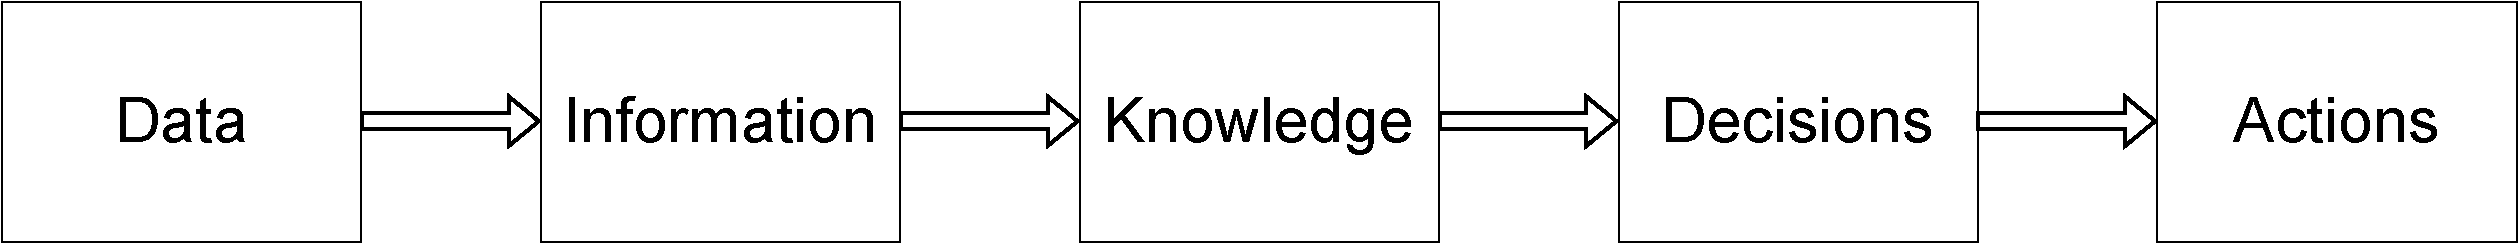
\includegraphics[width=0.99\textwidth, keepaspectratio]{content/02_theretical_foundations/informationValueChain.pdf}
    \caption{Information Value Chain}    
    \label{information_value_chain}
\end{figure}


